\documentclass[a4paper,12pt]{article}

% --- Packages ---
\usepackage{graphicx}
\usepackage{tikz}
\usepackage{geometry}
\usepackage{setspace}
\usepackage{titlesec}
\usepackage{everypage}
\usepackage{listings}
\usepackage{tcolorbox}

% --- Terminal View ---
\newtcolorbox{terminal}{
  colback=black!95,
  coltext=white,
  colframe=black,
  fontupper=\ttfamily,
  left=2mm, right=2mm, top=1mm, bottom=1mm,
  sharp corners
}
% --- Code style ---
\lstset{
  basicstyle=\ttfamily\small,
  backgroundcolor=\color{gray!10},
  frame=single,
  numbers=left,
  numberstyle=\tiny,
  keywordstyle=\color{green},
  commentstyle=\color{green!50!black},
  stringstyle=\color{orange},
  showstringspaces=false
}

% --- Page setup ---
\geometry{top=1in, bottom=1in, left=1in, right=1in}
\setstretch{1.3}

\begin{document}

% ================= COVER PAGE =================
\thispagestyle{empty}

% --- Border Frame ---
\AddEverypageHook{%
\begin{tikzpicture}[remember picture,overlay]
  \draw[line width=1pt]
    ([xshift=1cm,yshift=-1cm]current page.north west)
    rectangle
    ([xshift=-1cm,yshift=1cm]current page.south east);
  \draw[line width=0.5pt,dashed]
    ([xshift=1.2cm,yshift=-1.2cm]current page.north west)
    rectangle
    ([xshift=-1.2cm,yshift=1.2cm]current page.south east);
\end{tikzpicture}}

% --- University Logo & Name ---
\begin{center}
    
\includegraphics[width=5cm]{image.png}\\[0.5cm]
    {\LARGE \textbf{University of AJ\&K, Neelum Campus}} \\[0.3cm]
    {\Large Department of Computer Science \& IT} \\[0.8cm]
    \rule{0.75\textwidth}{1pt} \\[0.5cm]

    % --- Main Title (Subject + Assignment No) ---
    {\Large \bfseries Computer Organization and Assembly Language} \\[0.3cm]
    {\large \bfseries Assignment No. 3} \\[0.5cm]

    \rule{0.75\textwidth}{1pt} \\[1cm]
\end{center}

% --- Assignment Details ---
\begin{center}
    \Large \textbf{Topic} \\[0.3cm]
    Assembly Program to Print a Message
\end{center}

\vspace{3cm}

% --- Submitted By ---
\begin{center}
        \Large \textbf{Submitted By:} \\[0.3cm]
        Jawad Ahmed
\end{center}

% --- Footer with Date ---
\vfill
\begin{center}
    \rule{0.75\textwidth}{1pt} \\[0.3cm]
    {\large 4 Sept 2025} \\
\end{center}

\thispagestyle{empty}



% --- Title Page ---
\begin{titlepage}
    \centering
    \rule{\textwidth}{1pt} \\[0.5cm]
    {\Large \textbf{Course Information}}\\[0.2cm]
    \rule{\textwidth}{1pt} \\[1.2cm]
    
    \begin{tabular}{rl}
        \textbf{Course Name:} & Computer Organization and Assembly Language \\
        \textbf{Course Code:} & CSC-542 \\
        \textbf{Course Instructor:} & Abdual Qaddous \\
    \end{tabular}
    
    \vfill
    
    \rule{\textwidth}{1pt} \\[0.5cm]
    {\Large \textbf{Student Information}}\\[0.2cm]
    \rule{\textwidth}{1pt} \\[1.2cm]
    
    \begin{tabular}{rl}
        \textbf{Name:} & Jawad Ahmed Khawaja \\
        \textbf{Roll No:} & 04 \\
        \textbf{Semester:} & $BSCS-4^{th}$ \\
    \end{tabular}
    
    \vfill
    {\large \textbf{Submission Date:} 4-September-2025}
    
\end{titlepage}

\newpage
\centering
\rule{\textwidth}{1pt} \\[0.5cm]
    {\Large \textbf{Question}}\\[0.2cm]
\rule{\textwidth}{1pt} \\ [0.5cm]


Write down a program in Assembly Language to print the message of your own choice.
\rule{\textwidth}{1pt} \\[0.5cm]
    {\Large \textbf{Code}}\\[0.2cm]
\rule{\textwidth}{1pt} \\[1.2cm]


\begin{tcolorbox}[colback=white,colframe=black,title=Assembly Code]
\begin{verbatim}
.686
INCLUDE Irvine32.inc 
.data
    msg BYTE "Hello, from Assembly!",0
.code
    Main PROC
        lea edx, msg
        Call Clrscr
        Call WriteString
        EXIT
    Main ENDP
    END Main
\end{verbatim}
\end{tcolorbox}

\rule{\textwidth}{1pt} \\[0.5cm]
    {\Large \textbf{Output}}\\[0.2cm]
\rule{\textwidth}{1pt} \\[1.2cm]

\begin{center}
    \fbox{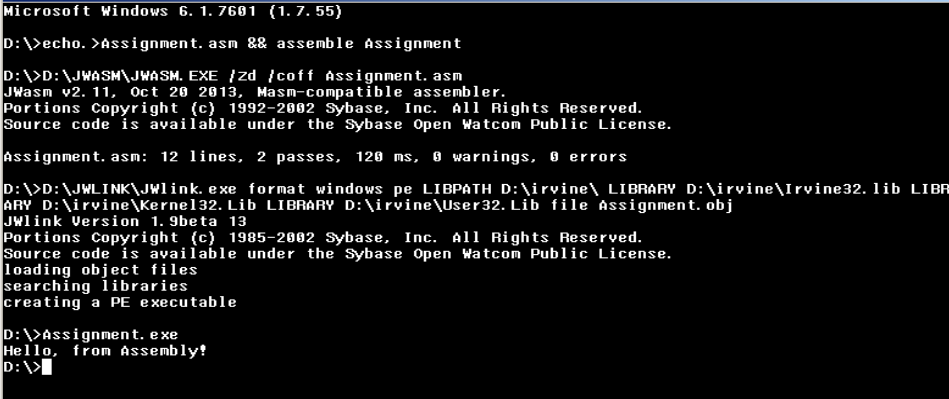
\includegraphics[width=9cm]{Ass.png}}
\end{center}

\newpage

\rule{\textwidth}{1pt} \\[0.5cm]
    {\Large \textbf{Explanations of Code}}\\[0.2cm]
\rule{\textwidth}{1pt} \\[1.2cm]


\begin{enumerate}
    \item \texttt{.686} \\
    This directive tells the assembler to generate code for the Intel 686 (Pentium Pro) processor or higher. It sets the instruction set architecture.

    \item \texttt{INCLUDE Irvine32.inc} \\
    This line includes the Irvine32 library, which provides useful procedures (like \texttt{WriteString}, \texttt{Clrscr}, etc.) for easier input/output operations in Assembly language.

    \item \texttt{.data} \\
    This section is used to declare initialized data or constants. Here we define variables that will be used in the program.

    \item \texttt{msg BYTE "Hello, from Assembly!",0} \\
    This defines a string variable named \texttt{msg}. The string is terminated with a null byte (0), which signals the end of the string.

    \item \texttt{.code} \\
    This marks the beginning of the code section where the instructions (executable code) are written.

    \item \texttt{Main PROC} \\
    It defines the beginning of the procedure (function) named \texttt{Main}. This is the entry point of the program.

    \item \texttt{lea edx, msg} \\
    It loads the effective address of the variable \texttt{msg} into the register \texttt{EDX}. The Irvine32 library procedures expect the address of the string in \texttt{EDX}.

    \item \texttt{Call Clrscr} \\
    It calls the procedure \texttt{Clrscr}, which clears the console screen.

    \item \texttt{Call WriteString} \\
    It calls the procedure \texttt{WriteString}, which prints the string located at the address in \texttt{EDX}.

    \item \texttt{EXIT} \\
    It ends the program and returns control to the operating system.

    \item \texttt{Main ENDP} \\
    It marks the end of the \texttt{Main} procedure.

    \item \texttt{END Main} \\
    It tells the assembler that the program execution should start at the label \texttt{Main}.
\end{enumerate}

\rule{\textwidth}{1pt} \\[0.5cm]
    {\Large \textbf{Flowchart of Program Execution}}\\[0.2cm]
\rule{\textwidth}{1pt} \\[1.2cm]


\begin{center}
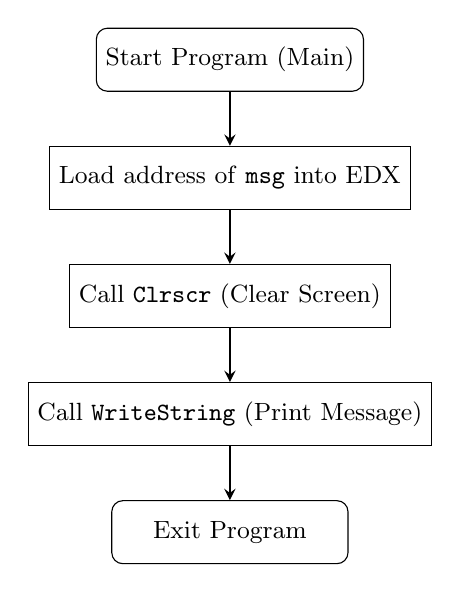
\begin{tikzpicture}[node distance=1.5cm, every node/.style={font=\small}]
\tikzstyle{startstop} = [rectangle, rounded corners, minimum width=3cm, minimum height=0.8cm,
text centered, draw=black, fill=white]
\tikzstyle{process} = [rectangle, minimum width=3cm, minimum height=0.8cm,
text centered, draw=black, fill=white]
\tikzstyle{arrow} = [thick,->,>=stealth]


% Nodes
\node (start) [startstop] {Start Program (Main)};
\node (load) [process, below of=start] {Load address of \texttt{msg} into EDX};
\node (clear) [process, below of=load] {Call \texttt{Clrscr} (Clear Screen)};
\node (print) [process, below of=clear] {Call \texttt{WriteString} (Print Message)};
\node (end) [startstop, below of=print] {Exit Program};

% Arrows
\draw [arrow] (start) -- (load);
\draw [arrow] (load) -- (clear);
\draw [arrow] (clear) -- (print);
\draw [arrow] (print) -- (end);
\end{tikzpicture}
\end{center}



\rule{\textwidth}{1pt} \\[0.5cm]
    {\Large \textbf{Summary}}\\[0.2cm]
\rule{\textwidth}{1pt} \\[1.2cm]
In this program, we learned how to display a simple message using Assembly Language. 
The program uses the \texttt{Irvine32.inc} library for input/output operations. 
This program demonstrates the basic structure of an Assembly Language program, 
including the use of data definition, procedure calls, and screen output.


\end{document}

